\section{Bài 03}

Xem xét bài toán
\begin{equation}
    \label{problem:03}
    \begin{aligned}
        \max \quad & x^2 + (y+1)^2\\
        \textrm{s.t.} \quad & -x^2 + y \geq 0\\
          &x + y \leq 2   \\
    \end{aligned}
\end{equation}
\begin{enumerate}[label=(\alph*)]
    \item Viết điều kiện FJ, và lập luận rằng $\lambda_0 \ne 0$
    \item Vẽ miền khả thi (feasible region), và bằng hình vẽ, xác định (các) lời giải tối ưu.
    \item Xác định tất cả các điểm mà thỏa mãn các điều kiện KKT; sau đó xác định các cực đại (toàn cục) giữa chứng.
\end{enumerate}


\begin{solution}

    Dựa trên nguyên lý đối ngẫu, ta viết lại bài toán như sau:
    \begin{equation}
        \begin{aligned}
            \min \quad & -x^2 - (y+1)^2\\
            \textrm{s.t.} \quad & x^2 - y \leq 0\\
              &x + y - 2\leq 0   \\
        \end{aligned}
    \end{equation}
    Các thành phần trong bài toán này như sau:
    \begin{align}
        \begin{aligned}
            f(x,y) &= -x^2 - (y+1)^2\\
            g_1(x,y) &= x^2 - y\\
            g_2(x, y) &= x + y - 2\\
        \end{aligned}
    \end{align}
    \begin{enumerate}[label=(\alph*)]
        \item Ta hình thành dạng yếu của hàm Lagrangian như sau:
        \begin{equation}
            L = -\lambda_0\left[x^2 + (y+1)^2\right] + \lambda_1(x^2 - y) + \lambda_2(x+y-2)
        \end{equation}
        Các điều kiện Fritz John (FJ) được viết như sau:
        \begin{itemize}
            \item \begin{equation}
                -2x\lambda_0 +2x\lambda_1 + \lambda_2 = 0 \Leftrightarrow x = \dfrac{\lambda_2}{2(\lambda_0 - \lambda_1)}
            \end{equation}
            \item \begin{equation}
                -2\lambda_0(y+1) -\lambda_1 + \lambda_2 = 0 \Leftrightarrow y = \dfrac{-2\lambda_0 - \lambda_1 + \lambda_2}{2\lambda_0},
            \end{equation}
            \item \begin{equation}
                \lambda_1 \geq 0, x^2 - y \leq 0, \lambda_1 (x^2 - y) = 0,
            \end{equation}
            \item \begin{equation}
                \lambda_2 \geq 0, x + y - 2 \leq 0, \lambda_2(x + y - 2) = 0
            \end{equation}
        \end{itemize}
        Nếu $\lambda_0 = 0$ thì biểu thức (3.6) không xác định. Do đó, $\lambda_0 \ne 0$.
        \item Vẽ miền khả thi (feasible region), và bằng hình vẽ, xác định (các) lời giải tối ưu.
        \begin{figure}[h!]
            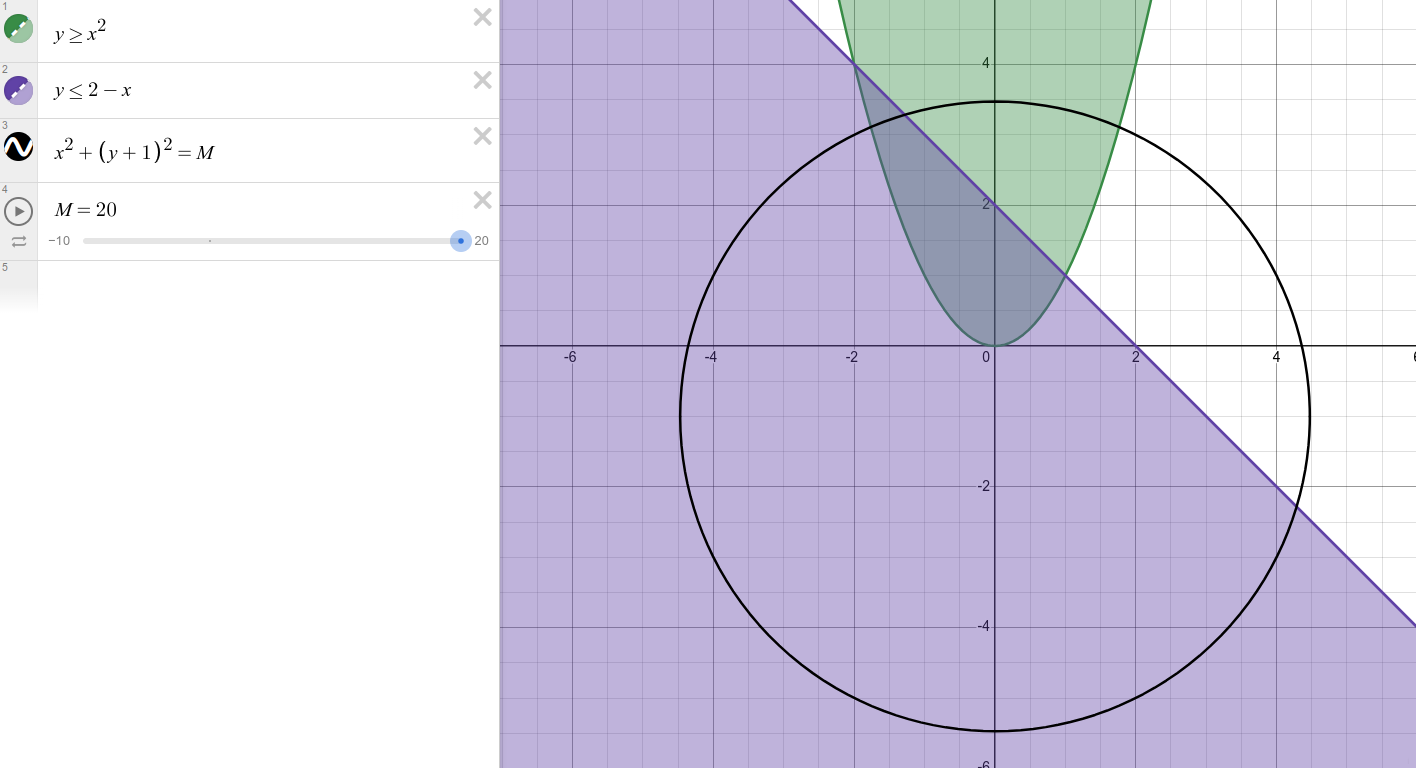
\includegraphics[width=0.85\linewidth]{figures/BT03.png}
            \caption{Miền khả thi của bài toán (\ref{problem:03}).}
            \label{fig:feasible_region_problem_03}
        \end{figure}
        \item Do $\lambda_ 0 \ne 0$, nên điều kiện KKT được thỏa mãn tại tất cả các điểm mà thỏa điều kiện FJ. Giả định rằng $\lambda_0 = 1$, ta có:
        \begin{equation}
            \begin{cases}
                x = \dfrac{\lambda_2}{2(1 - \lambda_1)} \\\\
                y = \dfrac{-2- \lambda_1 + \lambda_2}{2}
            \end{cases}
        \end{equation}
        Bằng cách kiểm tra các trường hợp
        \begin{enumerate}[label=(\roman*)]
            \item $\lambda_1 > 0$ và $\lambda_2 > 0$. Ta có hệ phương trình:
            \begin{equation}
                \begin{cases}
                    x^2 - y = 0 \\ 
                    x + y - 2 = 0
                \end{cases}
                \Leftrightarrow 
                \begin{cases}
                    x = 1 \\
                    y = 1
                \end{cases}
                \quad
                \text{hoặc}
                \quad
                \begin{cases}
                    x = -2 \\
                    y = 4
                \end{cases}
            \end{equation}
            Khi $(x, y) = (1, 1)$, ta giải được $(\lambda_1, \lambda_2) = \left(\dfrac{-2}{3}, \dfrac{10}{3}\right)$ nên điểm $(x, y) = (1, 1)$ không phải một điểm KKT. Và khi $(x, y) = (-2, 4)$, ta giải được $(\lambda_1, \lambda_2) = (14, 24)$ nên điểm $(x, y) = (-2, 4)$ là một điểm KKT.
            \item $\lambda_1 = 0$ và $\lambda_2 > 0$. Trong trường hợp này, thay $\lambda_1 = 0$, ta được:
            \begin{equation}
                \begin{cases}
                    x = \dfrac{\lambda_2}{2} \\\\
                    y = \dfrac{-2 + \lambda_2}{2}\\
                    x + y - 2 = 0
                \end{cases}
            \end{equation}
            Giải hệ này, ta được $\lambda_2 = 3$, $(x, y) = \left(\dfrac{3}{2}, \dfrac{1}{2}\right)$ là một điểm KKT.
            \item $\lambda_1 > 0$ và $\lambda_2 = 0$. Tương tự, ta thay $\lambda_2 = 0$, ta được:
            \begin{equation}
                \begin{cases}
                    x = 0 \\\\
                    y = \dfrac{-2- \lambda_1}{2}\\
                    y - 2 = 0
                \end{cases}
            \end{equation}
            Giải hệ này, ta được $\lambda_1 =- 6$, điểm $(x, y)$ trong trường hợp này không phải một điểm KKT.
            \item $\lambda_1 = 0$ và $\lambda_2 = 0$. Ta có được nghiệm $(x, y) = (0, -1)$
            là một điểm KKT.
        \end{enumerate}
        Các điểm KKT lần lượt là $(0, -1), (-2, 4), \left(\dfrac{3}{2}, \dfrac{1}{2}\right)$
    \end{enumerate}
\end{solution}
